\documentclass[a4paper,10pt,twoside,onecolumn,openright,leqno]{book}
\usepackage[doublespace]{thesis}
\usepackage{ist-thesis}
\usepackage[english]{babel}
\usepackage[utf8]{inputenc}
\usepackage[T1]{fontenc}
\usepackage[en-GB]{datetime2}

\usepackage[printonlyused,nohyperlinks]{acronym}
\usepackage{epstopdf}
\usepackage{fancyvrb}
\usepackage{url}


\usepackage[inline]{enumitem}
\usepackage{algorithm}
\usepackage{algpseudocode}
\usepackage{amsmath}
\usepackage{footnote}
\usepackage{graphicx}
\usepackage{listings}
\usepackage{mathtools}
\usepackage{natbib}
\usepackage{tabu}
\usepackage{tikz}
\usepackage{ulem}

\usepackage[hidelinks,bookmarks=true]{hyperref}

\renewcommand{\lstlistoflistings}{\begingroup
\tocfile{\lstlistlistingname}{lol}
\endgroup}

\lstset{ %
  backgroundcolor=\color{white},   % choose the background color
  basicstyle=\ttfamily,            % size of fonts used for the code
  breaklines=true,                 % automatic line breaking only at whitespace
  captionpos=b,                    % sets the caption-position to bottom
  commentstyle=\itshape\color{gray},  % comment style
  escapeinside={\%*}{*)},          % if you want to add LaTeX within your code
  keywordstyle=\color{blue},       % keyword style
  stringstyle=\color{red},         % string literal style
  numberstyle=\color{yellow},      % number literal style
}

% Fix lists so they do not have spacing between items
\setlist{noitemsep}

% Resets emph to italics instead of underline
\normalem

\usetikzlibrary{er,arrows,calc,shapes,positioning}

\usepackage{fancyhdr}

\fancypagestyle{plain}{
\fancyhf{}

\renewcommand{\headrulewidth}{0pt}
\renewcommand{\footrulewidth}{0pt}

\lfoot[\small\thepage]{}
\rfoot[]{\small\thepage}}

\title{SENTIDO: A Word Sense Induction Model\\ for Portuguese}
\author{José Pedro de Almeida Arvela}
\field{Computer Science and Engineering}
\supervisor{Prof. Nuno João Neves Mamede,\\ Prof. Jorge Manuel Evangelista
Baptista}

\chairperson{???}
\committeesup{???}
\committeemembers{???}

\begin{document}

\hypersetup{pageanchor=false}

\DTMlangsetup[en-GB]{showdayofmonth=false}
\maketitle
\DTMlangsetup[en-GB]{showdayofmonth=true}

\frontmatter
\hypersetup{pageanchor=true}
\cleardoublepage
\chapter*{Acknowledgements}
\addcontentsline{toc}{chapter}{Acknowledgements}
TODO

\cleardoublepage
\chapter*{Resumo}
\addcontentsline{toc}{chapter}{Resumo}
Com o crescer exponencial de informação publicada, processar a mesma torna-se
cada vez mais necessário. Desambiguação Semântica de Palavras é um componente
fundamental deste processo, mas não é possível sem corpora anotada com o sentido
de cada palavra em cada contexto. Indução Semântica de Palavras tenta resolver
este problema ao assumir que palavras no mesmo contexto estão semanticamente
relacionadas e ao criar aglomerados a partir de corpora não anotados.
\acf*{SENTIDO} é um novo projeto que tenta resolver este problema para a língua
portuguesa utilizando algoritmos com base em grafos.

\cleardoublepage
\chapter*{\abstractname}
\addcontentsline{toc}{chapter}{\abstractname}
With the exponential growth of data published, processing this data
automatically ever more necessary. \acf*{WSD} is a fundamental component of this
processing, but it is not possible without a rich sense inventory. \acf*{WSI}
tries to solve this problem by assuming words in the same context are
semantically related and creating clusters from unannotated corpora.
\acf*{SENTIDO} is a new project which attempts to solve this problem for the
Portuguese language using a graph-based algorithm.

\cleardoublepage
\phantomsection
\begin{keywords}
Natural Language Processing

Semantic Annotation

Sense Annotation

Text Analysis

Word Sense Disambiguation

Word Sense Induction

\bigskip
\bigskip

Processamento de Lingua Natural

Anotação Semântica

Anotação de Sentidos

Análise de Texto

Desambiguação Semântica de Palavras

Indução Semântica de Palavras
\end{keywords}

\cleardoublepage
\pdfbookmark{\contentsname}{Contents}
\tableofcontents

\cleardoublepage
\listoffigures

\cleardoublepage
\listoftables

\cleardoublepage
\lstlistoflistings

\cleardoublepage
\chapter*{Acronyms}
\addcontentsline{toc}{chapter}{Acronyms}

\begin{acronym}[RuDriCo2]
  \acro{AJAX}{Asynchronous JavaScript and XML}
  \acro{AP}{Almuhareb–Poesio}
  \acro{AR}{Anaphora Resolution}
  \acro{B-MST}{Balanced Maximum Spanning Tree}
  \acro{BNC}{British National Corpus}
  \acro{CBC}{Clustering By Committee}
  \acro{CSV}{Comma Separated Values}
  \acro{CW}{Chinese Whispers}
  \acro{DM}{Distributional Memory}
  \acro{DOM}{Document Object Model}
  \acro{DSM}{Distributional Semantic Model}
  \acro{EL}{Entity Linking}
  \acro{EM}{Expectation-Maximization}
  \acro{ER}{Entity--Relationship}
  \acro{GS}{Gold Standard}
  \acro{HAC}{Hierarchical Agglomerative Clustering}
  \acro{HMM}{Hidden Markov Model}
  \acro{IC}{Integrity Constraint}
  \acro{IR}{Information Retrieval}
  \acro{JC}{Jaccard Similarity Coefficient}
  \acro{LSA}{Latent Semantic Analysis}
  \acro{MARv}{Morphossyntactic Ambiguity Resolver}
  \acro{MFS}{Most Frequent Sense}
  \acro{ML}{Machine Learning}
  \acro{NER}{Named Entity Recognition}
  \acro{NLP}{Natural Language Processing}
  \acro{NMF}{non-negative matrix factorization}
  \acro{NPMI}{Normalized Pointwise Mutual Information}
  \acro{PHP}{PHP: Hypertext Preprocessor}
  \acro{PMI}{Pointwise Mutual Information}
  \acro{POS}{Part-of-Speech}
  \acro{RI}{Random Indexing}
  \acro{RNN}{Respective Nearest Neighbours}
  \acro{RuDriCo2}{Rule Driven Converter}
  \acro{SENTIDO}{SENse Through InDuctiOn}
  \acro{SGML}{Standard Generalized Markup Language}
  \acro{STRING}{Statistical and Rule-Based Natural Language Processing Chain}
  \acro{SVD}{Singular Value Decomposition}
  \acro{SWSI}{SemEval 2007 WSI task}
  \acro{WSD}{Word Sense Disambiguation}
  \acro{WSI}{Word Sense Induction}
  \acro{XIP}{Xerox Incremental Parser}
  \acro{XML}{Extensible Markup Language}

  \acroplural{DSM}[DSMs]{Distributional Semantic Models}
  \acroplural{HMM}[HMMs]{Hidden Markov Models}
  \acroplural{IC}[IC]{Integrity Constraints}

  \acroindefinite{SGML}{an}{a}
\end{acronym}
\newpage
% kate: default-dictionary en_GB; indent-width 2; replace-tabs on;
% kate: remove-trailing-space on; space-indent on;
% kate: replace-trailing-space-save on; remove-trailing-space on;


% Start the real document
\mainmatter
\pagestyle{plain}
\chapter{Introduction}

% Explain the problem

In human languages, it is possible that the same word has different meanings
according to the context in which it is used. For example:

\begin{enumerate}[label=(\alph*)]
 \item She shot the arrow using her \textit{bow}.
 \item He tied the \textit{bow} of the gift.
\end{enumerate}

In these two sentences, the word \textit{bow} means different things. In
sentence (a) it is used as a hunting tool, while in sentence (b) it is a ribbon.
To be able to do some tasks in \ac{NLP}, machines need to be able to
differentiate between each use of the same word.

% Show why the problem is ubiquitous

This problem affects, among other \ac{NLP} tasks, \ac{MT}, \ac{IR} and content
categorization \citep{navigli2009word}. Taking an example from \ac{MT}, the
Portuguese word \textit{laço} can be translated in various different English
words depending on context; it can be translated into \textit{ribbon} or it can
be translated to the \textit{bond} between two people. A system which naïvely
uses the \ac{MFS} may improperly translate or categorize this word when it is
used outside of its most common context.

% Introduce the solution to the problem

To deal with this problem it is necessary to identify the underlying meaning of
a word based on its context. This process is called \ac{WSD}
\citep{navigli2009word}. This process requires both sense inventories as well as
large amounts of sense-tagged \emph{corpora} to function efficiently. As a
result, under-resourced languages need to deal with greater hardships to be
able to achieve satisfactory results \citep{ng1997getting}.

A solution to the lack of resources is to automatically identify the meaning of
words in their given context, without the requirement of manually annotated
data. This is called \ac{WSI} \citep{agirre2007semeval}.

% Propose questions which this paper will answer

% Is it possible?
% Does it execute within reasonable limits?
% Can it be better than no induction/disambiguation?
% How do you evaluate it? Aka, how do you know it is better?

The goal of this dissertation is to investigate the feasibility of creating a
\ac{WSI} model for the Portuguese language which is capable of improving the
quality of detected word senses within the words' contexts. Furthermore, this
dissertation looks into seeing if the task of \ac{WSI} and \ac{WSD} can be
performed within reasonable time, and to evaluate the quality of this new model
against the \ac{MFS} baseline.

% Introduce the shiny new tool, explain the problem it solves

Additionally, this dissertation presents the results of this investigation, in
a project called \ac{SENTIDO}. \ac{SENTIDO} is a \ac{WSI} and \ac{WSD} model
which infers the possible senses of a word from untagged \emph{corpora} based
on the additional words that co-occur with the target word; and, given a word
and its context, disambiguates between the previously inferred senses.

% Describe the layout of this paper

This dissertation is organized as follows:

In Chapter~\ref{ch:stateofart}, existing \ac{WSI} implementations and models
are described, as well and the theoretical foundations and additional tools
that support and aide them. In Chapter~\ref{ch:architecture}, the architecture
of the model is outlined, as well as the various stages that compose it. In
Chapter~\ref{ch:implementation}, the implementation details, such as the
\emph{corpora} used, existing tools from which the model is developed, and
adaptations made to those same tools, are depicted.
Chapter~\ref{ch:eval-method} describes how the algorithm is tested and which
are the theoretical foundations for the soundness of the methodology.
Chapter~\ref{ch:eval} describes the test corpus used, the chosen parameters and
analyses the results of the evaluation. Chapter~\ref{ch:conclusion} provides a
synopsis of the findings and describes what can be improved in the future.

% kate: default-dictionary en_GB; indent-width 2; replace-tabs on;
% kate: remove-trailing-space on; space-indent on;
% kate: replace-trailing-space-save on; remove-trailing-space on;

\chapter{State of the Art}
\label{sec:stateofart}

In this section the state of the art is described. The overall approaches and
their principles are described, as well as the various algorithms used to
exploit those same principles.

\section{Distributional Semantics}

\acp{DSM} discover word senses from text. These are based on the
\textit{Distributional Hypothesis}, which says that \textit{similar terms
appear in similar contexts} \cite{curran2004distributional}. That is, words are
semantically similar if they appear in similar documents, context windows or
syntactic contexts \cite{van2010mining}.

Using syntactic contexts adds a restriction to what can be considered context of
a word. For a word to be in the context of another, it needs to be linked
through the use of a relevant syntactic or lexical relation
\cite{baroni2010distributional}.

\section{Statistical and Vector Space Models}
\label{sec:vectorspace}

These methods implement \acp{DSM} either based on a statistically or a 
geometrically  oriented probability distribution models \citep{van2010mining}. 
Some of these methods are presented below.

\subsection{\acl*{CBC}}

An implementation of a clustering approach is \ac{CBC} 
\citep{pantel2003clustering}. The algorithm represents each word as a feature 
vector, in which each feature corresponds to a context where the word occurs. 
The value of the feature is the \ac{PMI} between the feature and the word 
\citep{bouma2009normalized}, which is later described in \ref{subsec:pmi}. The 
similarity between two words is computed using the \textit{cosine coefficient} 
\citep{salton1986introduction} of their mutual information vectors, as in 
Equation~\ref{eq:simwiwj}.

\begin{equation}
\operatorname{sim}(w_i,w_j) = \frac{\sum_c mi_{w_i,c} \times mi_{w_j,c}}
                    {\sqrt{\sum_c{mi_{w_i,c}}^2 \times \sum_c{mi_{w_j,c}}^2}}
\label{eq:simwiwj}
\end{equation}

The \ac{CBC} algorithm consists of three phases. In phase I, the top-$k$ 
similar elements of each element $e$ are computed. In phase II a collection of 
tight clusters is constructed, where the elements of each cluster form a 
committee. In each step, the algorithm finds a set of tight clusters, called 
committees, and identifies residue elements not covered by any. First the 
top-$k$ similar elements are clustered using average-link clustering 
\citep{han2000data}. A committee covers an element if its similarity to the 
centroid of the committee exceeds a given threshold. The algorithm then 
recursively attempts to find more committees among the residue elements. The 
details are presented in Algorithm~\ref{alg:cbcphaseii}.

\begin{algorithm}
\begin{algorithmic}
\Function{phaseII}{$E$, $S$, $\theta_1$, $\theta_2$}
  \ForAll {$e \in E$}
    \State $C \gets$ \Call{average-link}{$S$, $e$}
    \ForAll {$c \in C$}
      \Comment{For each cluster discovered}
      \State $Sc(c) \gets |c| \times $ \Call{avgsim}{$c$}
      \Comment{Compute its score}
    \EndFor
    \State $L \gets L \cup c \in C, \max(Sc) = c$
    \Comment{Store highest-scoring cluster in a List L}
  \EndFor

  \State $L \gets$ \Call{sort}{$L$}

  \State $C \gets$ \Call{new-list}{}
  \Comment{List of committees}
  \ForAll {$c \in L$}
    \State $cn \gets$ \Call{centroid}{c}
    \If {$\forall c' \in C, sim(c, $ \Call{centroid}{$c'$} $) < \theta_1$}
      \State $C \gets C \cup c$
    \EndIf
  \EndFor

  \If {$C \subset \emptyset$}
    \State \Return $C$
  \EndIf

  \State $R \gets$ \Call{new-list}{}
  \Comment{List of Residues}
  \ForAll {$e \in E$}
    \If {$\forall c \in C, sim(e, c) < \theta_2$}
      \State $R \gets R \cup e$
    \EndIf
  \EndFor

  \If {$R \subset \emptyset$}
    \State \Return $C$
  \Else
    \State \Return $C \cup$ \Call{phaseII}{$R$, $S$, $\theta_1$, $\theta_2$}
  \EndIf
\EndFunction
\end{algorithmic}
\caption{\label{alg:cbcphaseii} Phase II of CBC}
\end{algorithm}


In phase III each element $e$ is assigned to its most similar clusters
according to Algorithm~\ref{alg:cbcphaseiii}. The similarity between a cluster
and an element is computed using the centroid of the committee members. Once an
element $e$ is assigned to a cluster $c$, the intersecting features between
both are removed from $e$ to allow \ac{CBC} to discover the less frequent
senses of a word and avoid duplicate senses.

\begin{algorithm}
\begin{algorithmic}
\State $C$ is a list of clusters initially empty
\Function{phaseIII}{$e$}
  \State $S \gets$ \Call{top200}{$e$}
  \Comment{The top-200 similar clusters to e}

  \While {$\neg S \subset \emptyset$}
    \State $c \gets$ \Call{most-similar}{$S$, $e$}
    \If {$sim(e, c) < \sigma$}
      \State \textbf{break}
    \EndIf
   \If {$\forall c' \in C, \neg similar(c,c')$}
     \State $c \gets c \cup e$
     \State Remove from e its features that overlap with the features of c
   \EndIf
   \State $S \gets S \setminus \{c\}$
  \EndWhile
  \State \Return $C$
\EndFunction
\end{algorithmic}
\caption{\label{alg:cbcphaseiii} Phase III of CBC}
\end{algorithm}

To evaluate the system, its output was compared with WordNet, with the
frequency counts for the nodes, called synsets, obtained from the SemCor corpus 
\citep{miller1993semantic}.

The corpus was obtained by processing 144 million words of newspaper text from 
the TREC Collection (1988 AP Newswire, 1989-90 LA Times, and 1991 San Jose 
Mercury)\footnote{\url{http://trec.nist.gov/data/test_coll.html}, last 
accessed on \DTMdate{2017-09-28}.}. The test set was constructed by 
intersecting the words in WordNet 
with the nouns in the corpus, resulting in a test set of 13403 words with an 
average number of 740.8 features per word. \ac{CBC} obtained a precision of 
$60.8\%$, a recall of $50.8\%$ and an F-score of $55.4\%$. These evaluation 
measures are later described in Section~\ref{subsec:unsupeval}.

\subsection{HERMIT}

The model from \citet{jurgens2010hermit} performs \ac{WSI} by modelling 
individual contexts in a high dimensional word space. Word senses are induced 
by finding contexts which are similar and a hybrid clustering method is used to 
group similar contexts.

Each context of a word is approximated using the \ac{RI} word space model
\citep{kanerva2000random}, in which the occurrence of a word is represented with
an \textit{index vector} instead of a set of dimensions.

\ac{RI} can be described as a two-step operation
\citep{sahlgren2005introduction}:

\begin{enumerate}
 \item Each context in the data is assigned an unique and randomly generated
 representation, called an \textit{index vector}, which is sparse and
 high-dimensional. Its dimensionality ($d$) is on the order of thousands and
 it consists of a small number of randomly distributed values of $\pm1$, with 
 the rest of the elements set to $0$;
 \item Then, context vectors are produced by scanning through the text. Each
 time a word occurs in a context, the context's $d$-dimensional index vector is
 added to the context vector for that word. Words are represented by
 $d$-dimensional context vectors which are the sum of the words' contexts.
\end{enumerate}

This allows for a creation of a co-occurrence matrix $F_{w \times d}$ which is
an approximation of a standard co-occurrence matrix $F_{w \times c}$, but in
which $d \ll c$. As a result, HERMIT transforms the original co-occurrence 
counts into a smaller and denser representation without the computational 
overhead of other dimensional reduction techniques such as \ac{SVD} 
\citep{jurgens2010hermit}.

The identification of related contexts is made through the use of clustering, 
which separates similar context vectors into dissimilar clusters representing 
the distinct senses of a word. A hybrid of the online $k$-means clustering 
\citep{liberty2016algorithm} and \ac{HAC} \citep{zepeda2013hierarchical} with a 
threshold is used. The threshold allows for the number of clusters to be 
determined by data similarity instead of manually specified.

The context vectors are clustered using $k$-means clustering, which assigns a 
context to the most similar cluster centroid. If the nearest centroid has a 
smaller similarity than the \textit{cluster threshold} and there are not any 
$k$ clusters, the context forms a new cluster. The similarity between context 
vectors is defined as the cosine similarity (see above).

Clusters are then repeatedly merged using \ac{HAC} with average link criteria,
that is, cluster similarity is the mean cosine similarity of the pairwise
similarity of all data points from each cluster. When the two most similar
clusters have a similarity less than the threshold, merging stops. The resulting
clusters should then represent distinct word senses.

The model was submitted for SemEval-2010 Task 14 \citep{manandhar2009semeval}
and evaluated in an unsupervised method, which compares the found clusters with 
the gold data for the word senses, and a supervised method, which evaluates the 
results of \ac{WSD} using the induced clusters. The first was measured
according to the F-score and V-measure, which is the harmonic mean between the 
homogeneity and completeness (later described in Section~\ref{subsec:unsupeval});
while the second was measured using supervised recall. Using the provided test 
corpus, parameters were tuned for a context window size of $\pm1$, a clustering
threshold of $.15$ and a maximum of $15$ clusters per word.

The final results of the SemEval-2010 Task 14 showed that Hermit achieved a
V-measure of $16.7\%$ and an F-score of $24.4\%$ in nouns in the unsupervised
evaluation and a supervised recall of $53.6\%$.


% kate: default-dictionary en_GB; indent-width 2; replace-tabs on;
% kate: remove-trailing-space on; space-indent on;
% kate: replace-trailing-space-save on; remove-trailing-space on;

\section{Co-occurrence Graph Models}

In graph-based models, the meanings of a word are represented by a weighted
and undirected co-occurrence graph. The nodes (or vertices) of the graph are the
words which occur in the corpus and the edges are co-occurrences, with the
weight of the edge describing the amount of times that co-occurrence exists. Two
words are said to co-occur if they both occur within the same context.

These models are based on the idea that co-occurrence graphs have the properties
of \textit{small world networks} \cite{veronis2004hyperlex}, that is, most nodes
are not neighbours to one another, but most nodes can be reached by a small
number of steps, as shown in Figure~\ref{fig:small-world}. These properties
then allow to search for highly interconnected bundles of co-occurrences, that
is, \textit{high density components}, which correspond to the senses being
searched.

\begin{figure}
 \centering
 \includegraphics[width=0.5\textwidth]{graphics/small_world}
 \caption{An example of a small world network.}
 \label{fig:small-world}
\end{figure}

\subsection{Graph Model for Unsupervised Lexical Acquisition.}

A graph from a \ac{POS}-tagged corpus is made in \cite{widdows2002graph}, using
words as nodes and the grammatical co-occurrence relationships between pairs as
edges. The relationships extracted are the co-occurrences of Noun-Verb,
Verb-Noun, Adjective-Noun, Noun-Noun. To generate the edges the top-$n$
neighbours of each word are selected and turned into edges.

An incremental algorithm is then used to extract categories based on a given
word using affinity scores, which give more importance to words that are linked
to the existing neighbours. The algorithm is tailored to avoid infections from
spurious co-occurrences, preventing spurious links from relating to genuine
semantic similarity. The process to select and add the most similar node to a
set of nodes is described in Algorithm~\ref{alg:similarnodes}, where $A$ is a
set of nodes and $N(a)$ are all the nodes which are linked to a node $a$.

\begin{algorithm}
 \begin{algorithmic}
  \State $N(A) \gets \cup_{a \in A} N(a)$
  \State $b \gets u \in N(A) \setminus A, max(\frac{|N(u) \cap N(A)|}{|N(u)|})$
  \State $A \gets A \cup b$
 \end{algorithmic}
 \caption{\label{alg:similarnodes} Select the most similar node}
\end{algorithm}

The model was built using the \ac{BNC} and evaluated against classes in
WordNet. A WordNet class was considered to be the collection of synsets
subsumed by a parent synset. For a given seed word, the algorithm in
\ref{alg:similarnodes} was used to find the $n$ nodes most closely related to
it. Ten classes were chosen beforehand, and for each class 20 words were
retrieved using a single seed-word from the class in question.

The results show that of a total of 200 retrieved words, only 36 were
incorrect, giving an accuracy of $82\%$.

\subsection{Word Sense Induction Using Graphs of Collocations.}
\label{sec:collocations}

A graph of collocations is used in \cite{klapaftis2008word} to generate a
taxonomy of senses which takes into consideration word polysemy. In this, each
node corresponds to an occurrence of two words in the same context window (which
in the model is a paragraph) and two nodes are connected if two collocations
occur in the same context window.

The base corpus, $bc$, consists of paragraphs containing the target word, $tw$.
Besides $bc$, there is also a large reference corpus, $rc$. The project focuses
in inducing the sense of $tw$ given $bc$ as the only input.

At first, paragraphs with $tw$ are removed from $bc$ and all paragraphs from
$bc$ and $rc$ are \ac{POS} tagged. From these, only nouns are kept and
lemmatised.

Log-likelihood ($G^2$) is then used to filter common nouns which are not
semantically related to $tw$, by checking if a given word $w_i$ has a similar
distribution in $bc$ and $rc$. If that is true, $G^2$ will have a small value
and $w_i$ should be removed from $bc$.

\begin{equation}\label{eq:g2}
 G^2 = 2 * \sum_{i,j} n_{i,j} \cdot log \frac{n_{ij}}{m_{ij}}
\end{equation}

\begin{equation}\label{eq:mij}
 m_{ij} = \frac{\sum_{k=1}^2 n_{ik} \cdot \sum_{k=1}^2 n_{kj}}
               {N}
\end{equation}

The noun frequencies of $bc$ are stored in a list $lbc$ and the noun
frequencies of $rc$ are stored in a list $lrc$.

For each word $w_i \in lbc$ is created a table of observed counts from $lbc$
and $lrc$, OT, and a table of expected values under the model of independence,
ET. $G^2$ is then calculated (Equation~\ref{eq:g2}), where $n_{ij}$ is the
$i,j$ cell of OT and $m_{ij}$ (Equation~\ref{eq:mij}) is the $i,j$ cell of ET,
and $N = \sum_{i,j} n_{ij}$.

$lbc$ is then filtered by removing words with a smaller relative frequency in
$lbc$ in relation to $lrc$. The resulting $lbc$ is then sorted by the $G^2$
values. Words that have a $G^2$ smaller than a pre-specified threshold $p_1$
are then removed from $bc$. By the end of this process, each paragraph in $bc$
is a list of nouns assumed to be topically related to $tw$.

With the base corpus now processed, collocations of two nouns are detected by
generating all $\binom{n}{2}$ combinations for each $n$-length paragraph.
Conditional probabilities (Equation~\ref{eq:pij}) are then used to generate the
weights of each collocation. Collocations that have a frequency and weight
higher than a pre-specified threshold are then used to generate the nodes of the
graph $G$.

\begin{equation}\label{eq:pij}
 p(i|j) = \frac{f_{ij}}{f_{j}}
\end{equation}

The constructed graph $G$ is sparse. A smoothing technique is applied to
discover new edges between vertices and to assign weight to all of the graph's
edges. For each vertex $i$, a vertex vector $VC_i$ is assigned containing the
vertices which share an edge with $i$ in $G$. The similarity between each $VC_i$
and $VC_j$ is then calculated using the \ac{JC} (Equation~\ref{eq:jc}).

\begin{equation}\label{eq:jc}
 JC(VC_i, VC_j) = \frac{|VC_i \cap VC_j|}
                       {|VC_i \cup VC_j|}
\end{equation}

The final graph, $G'$, is then clustered using \ac{CW}, further described in
Section~\ref{sec:cw}. This algorithm was used as it does not require input
parameters and performs in linear time to the number of edges, although it is
not guaranteed to converge.

\ac{WSD} is at last made by assigning one of the induced clusters to each
instance of the target word. For each target word in a given paragraph, a score
for each induced cluster is applied, based on the number of collocations which
occur in the paragraph.

For the part of \ac{WSD}, for each paragraph of $bc$, each induced cluster is
assigned a score equal to the number of collocations occurring in it.

To evaluate the model, the framework of the \ac{SWSI} \cite{agirre2007semeval}
was used. The test corpus consists of texts from the Wall Street Journal
corpus, hand-tagged with OntoNotes senses \cite{hovy2006ontonotes}.

The model was evaluated under \textit{unsupervised evaluation}, where the
resulting classes are compared to the \ac{GS}, and under \textit{supervised
evaluation}, where the model's performance on a \ac{WSD} setting with the
test corpus is measured.

The model was evaluated with and without smoothing. In the unsupervised
evaluation, the model with smoothing achieved $88.6\%$ purity, $31\%$ entropy
(these measures are described below, in Section~\ref{sec:unsupeval}) and an
F-Score of $78.0\%$. Results without smoothing were similar, but with a lower
F-Score due to the larger number of induced clusters.

\subsection{UoY: Graphs of Unambiguous Vertices.}

The model developed in \cite{korkontzelos2010uoy} is a relaxed version of the
model in \cite{klapaftis2008word}, described in Section~\ref{sec:collocations},
in which a node is generated from a single word if it is considered unambiguous,
and a node is only generated from a set of two words if otherwise.

The corpus is first preprocessed, with the aim of capturing words contextually
related to the target. Sentences or paragraphs, \textit{snippets}, which contain
the target word are lemmatised and \ac{POS} tagged using the GENIA tagger. Only
nouns are kept and words which occour in a stoplist are filtered out. Nouns
which are infrequent in the reference corpus are removed and the log-likelihood
ratio ($G^2$) is used to compare the distribution of each noun to its
distribution in the reference corpus. If a noun's $G^2$ is lower than a
specified threshold, or the noun has a higher relative frequency in the
reference corpus than in the target corpus, then that noun is removed. At this
stage, each snippet is a list of lemmatised nouns contextually related to the
target word.

The graph is constructed by first representing all nouns in the list as graph
vertices. Each noun within a snippet is combined with every other, generating
$\binom{n}{2}$ pairs. $G^2$ is applied once again, to the pairs to filter out
unimportant ones.

To filter out pairs which refer to the same sense, a vector with the snippet IDs
in which they occur is generated for each pair and each noun. A pair is
discarded if its vector is similar to both vectors of their component nouns,
using for that purpose the Dice coefficient defined in Equation~\ref{eq:dice}.

\begin{equation} \label{eq:dice}
 QS = \frac{2 |X \cap Y|}{|X| + |Y|}
\end{equation}

Edges are drawn based on the co-occurrence of the corresponding vertices in
snippets. The weight of the edge is the maximum of the conditional probabilities
of its vertices, calculated according to Equation~\ref{eq:wab}, and low weighted
edges are filtered out.

\begin{equation} \label{eq:wab}
 w_{a,b} = \frac{1}{2} \left( \frac{f_{a,b}}{f_a} + \frac{f_{a,b}}{f_b} \right)
\end{equation}

The graph is then clustered using \ac{CW}, described in Section~\ref{sec:cw}.
To reduce the number of clusters, a post-processing stage is applied in which
for each cluster $l_i$, a set of all snippets $S_i$ containing at least one
vertex of $l_i$ is generated. For any clusters $l_a$ and $l_b$, if
$S_a \subseteq S_b$  or $S_a \supseteq S_b$, these are merged.

The model was submitted for SemEval-2010 Task 14 \cite{manandhar2009semeval}
and evaluated in an unsupervised and a supervised method. The first was measured
according to the V-measure and F-score, while the second was measured using
recall. Parameters were tuned by choosing maximum supervised recall, resulting
in threshold frequencies of 10, $G^2$ threshold of 10, collocations weights of
0.4 and similarity threshold for pairs-of-nouns vertices of 0.8.

Results showed that the model achieved results of a V-measure of $20.6\%$, an
F-score of $38.2\%$ on the unsupervised evaluation with nouns and a recall of
$59.4$ on the supervised evaluation.

% kate: default-dictionary en_GB; indent-width 2; replace-tabs on;
% kate: remove-trailing-space on; space-indent on;
% kate: replace-trailing-space-save on; remove-trailing-space on;

\section{Graph Partitioning and Clustering Algorithms}
\label{sec:clusteralgorithms}

The task of finding clusters which are optimal with respect to fitness measures
is NP-complete \citep{sima2006np}. The following are two current algorithms,
time-linear to the number of edges, which try to find solutions through
approximation.

\subsection{Chinese Whispers.}
\label{sec:cw}

\ac{CW} is a randomised graph-clustering algorithm which is time-linear in the
number of edges, developed by Biemann \citep{biemann2006chinese}. It is a basic,
yet effective, algorithm to partition nodes of weighted, undirected graphs, and
it is said to perform well in small-world graphs.

\ac{CW} is parameter-free, as the number of partitions emerges naturally during
the process. But formally, \ac{CW} does not converge, as a node can become tied
and be randomly assigned a different class at each iteration, without ever
stabilising, nor is it deterministic, due to the random orders and assignments
in the algorithm.

In \ac{CW}, a weighted graph, $G=(V,E)$, has nodes $v_i \in V$ and weighted
edges $(v_i, v_j, w_{ij}) \in E$ with weight $w_{ij}$. If $(v_i, v_j, w_{ij})
\in E$ implies $(v_j, v_i, w_{ij}) \in E$ then $G$ is undirected. If all weights
are 1, $G$ is unweighted. The degree of a node is the number of edges it takes
part in. The neighbourhood of a node $v$ is the set of all nodes $v'$ such that
$(v,v',w) \in E$ or $(v',v,w) \in E$.

\ac{CW} works as outlined in Algorithm~\ref{alg:cw}. First, all nodes get
different classes. For a small number of iterations, in each iteration, the
nodes inherit the strongest class in their neighbourhood. This is the class
whose sum of edge weights to the current node is maximal. If multiple classes
are equally the strongest, one is chosen randomly. Classes are updated
immediately, a node can obtain classes introduced in that same iteration.

Regions of the same class stabilize during the iteration, and grow until they
reach the border of another class.

\begin{algorithm}
 \caption{The Chinese Whispers algorithm}
 \label{alg:cw}
 \begin{algorithmic}
  \Function{ChineseWhispers}{V, E}
   \ForAll{$v_i \in V$}
    \State $class(v_i) \gets i$
   \EndFor

   \While{changes}
    \ForAll{$v \in V$, random order}
     \State $class(v) \gets max\_rank(class(neighbourhood(v)))$
    \EndFor
   \EndWhile
  \EndFunction
 \end{algorithmic}
\end{algorithm}

Apart from ties, the class of a node usually does not change more than a few
times. The number of iterations depends on the larger distance between two nodes
in the graph.

\ac{CW} was evaluated on tasks of \ac{WSI} using a similar approach to the one
in \citep{dorow2003discovering}, by replacing the Markov Clustering algorithm
with \ac{CW}. The evaluation method in \citep{bordag2006word} was used. In this,
the neighbourhood of two words is merged and the ability of the algorithm to
separate the merged graph is evaluated. The evaluation measures used included
\textit{retrieval precision} ($rP$), the similarity of the found sense with the
gold standard sense using the overlap measure, and the \textit{retrieval recall
($rR$)}, which are the amount of words assigned correctly to the gold standard
sense.

Results for nouns showed that \ac{CW} had a retrieval precision of $94.8\%$ and
a retrieval recall of $71.3\%$, which suggest similar performance as specialized
graph-clustering algorithms for \ac{WSI} given the same input.

\subsection{MaxMax.}
\label{sec:maxmax}

MaxMax is a soft-clustering algorithm applicable to edge-weighted graphs
\citep{hope2013maxmax}. It is parameter-free, runs in linear time to the number
of edges and it is deterministic. Test results show it to return scores
comparable with existing state-of-the-art systems.

In MaxMax, a notion of \textit{maximal affinity} is used, in which affinity
between vertices $u$ and $v$ is the edge weight $w(u,v)$. A vertex $u$ has
maximal affinity to a vertex $v$ if $w(u,v)$ is maximal among all edges with
$u$. $v$ is said to be a \textit{maximal vertex of $u$}.

MaxMax consists of two stages, as described in Algorithm~\ref{alg:maxmax}.
First, the weighted graph $G$ is transformed in an unweighted, directed graph
$G'$. Maximal affinity relationships between vertices are used to determine edge
direction in $G'$. If in $G$ a vertex $u$ has two maximal vertexes $v$ and $w$,
in $G'$ $u$ will have only two directed edges, from $v$ to $u$ and from $w$ to
$u$.

Then, clusters are identified, finding the \textit{root} vertices of subgraphs
of $G'$ and by marking all descendants of a vertex as $\neg root$. In the
directed graph $G'$, a vertex $v$ is a \textit{descendant} of $u$ is there is a
directed path from $u$ to $v$. At the end of the stage, vertices which are still
marked as $root$ uniquely identify clusters.

\begin{algorithm}
 \caption{The MaxMax algorithm}
 \label{alg:maxmax}
 \begin{algorithmic}
  \Function{MaxMax}{V, E}
   \ForAll{$(u,v) \in E$}
    \If{$v$ is $maximal\_vertex(u)$}
     \State $E' \gets E' \cup (v,u)$
    \EndIf
   \EndFor
   \State $G' \gets dirgraph(V, E')$
   \State $\forall v \in V, v \gets root$

   \ForAll{$v \in V$}
    \If{$v$ is $root$}
     \ForAll{$u \in descentant(v)$}
      \State $u \gets \neg root$
     \EndFor
    \EndIf
   \EndFor
  \EndFunction
 \end{algorithmic}
\end{algorithm}

MaxMax was evaluated in the context of the SemEval 2010 \ac{WSI} Task
\citep{manandhar2010semeval}, using an adaptation of the Shared Nearest
Neighbours algorithm and then using MaxMax to identify sense clusters in the
generated target word graph. MaxMax has the best scoring V-measure (of $32.8\%$)
among the systems evaluated in \citep{manandhar2010semeval}, and the worst
F-score (of $13.2\%$) among the systems evaluated. The authors claim that their
system is overly penalized by the F-score due to the way this is known to be
biased towards clustering solutions returning large clusters and to punish small
clusters disproportionately.

% kate: default-dictionary en_GB; indent-width 2; replace-tabs on;
% kate: remove-trailing-space on; space-indent on;
% kate: replace-trailing-space-save on; remove-trailing-space on;

\section{Other Tools}

In addition to the existing work in \ac{WSD} and \ac{WSI}, it is relevant to
mention other works which make use of word co-occurrences in text.

\subsection{STRING}
\label{sec:string}

\ac{STRING} \cite{mamede2012string} is a \ac{NLP} system for the Portuguese
language, capable of preforming all basic \ac{NLP} tasks, including \ac{NER},
\ac{IR}, \ac{AR}, among other tasks. \ac{STRING} is composed of several stages,
as described in Figure~\ref{fig:stringarch}.

\begin{figure}[ht]
 \caption{\acs*{STRING} Architecture}
 \label{fig:stringarch}
 \centering
 \tikzstyle{block} = [rectangle, draw, node distance=1.5cm,
    text width=2.5cm, text centered, minimum width=3cm, minimum height=3em,
    rotate=90, anchor=base]
\tikzstyle{line} = [draw, -latex']

\begin{tikzpicture}[node distance = 2cm, on grid]

  \node [block] (lexman) {LexMan};
  \node [block, below of=lexman] (rudrico) {RuDriCo2};
  \node [block, below of=rudrico] (marv) {MARv4};
  \node [block, below of=marv] (xip) {XIP};
  \node [block, below of=xip] (anaphora) {Anaphora Resolution};
  \node [block, below of=anaphora] (time) {Time Normalization};
  \node [block, below of=time] (slot) {Sloft Filling};
  \node [block, below of=slot] (event) {Event Ordering};
  \node [block, below of=event, ellipse, text width=1cm] (join) {Join};

  \path [line] ([xshift=-0.5cm]lexman.north) -- (lexman);

  \path [line] (lexman) -- (rudrico);
  \path [line] (rudrico) -- (marv);
  \path [line] (marv) -- (xip);

  \path [line] (xip) -- ([yshift=1cm]xip.east) --
               ([yshift=1cm]anaphora.east) -- (anaphora);
  \path [line] (xip) -- ([yshift=1cm]xip.east) --
               ([yshift=1cm]time.east) -- (time);
  \path [line] (xip) -- ([yshift=1cm]xip.east) --
               ([yshift=1cm]slot.east) -- (slot);
  \path [line] (xip) -- ([yshift=1cm]xip.east) --
               ([yshift=1cm]event.east) -- (event);
  \path [line] (xip) -- ([yshift=1cm]xip.east) --
               ([yshift=1cm]join.east) -- (join);

  \path [line] (anaphora) -- ([yshift=-1cm]anaphora.west) --
               ([yshift=-1cm]join.west) -- (join);
  \path [line] (time) -- ([yshift=-1cm]time.west) --
               ([yshift=-1cm]join.west) -- (join);
  \path [line] (slot) -- ([yshift=-1cm]slot.west) --
               ([yshift=-1cm]join.west) -- (join);
  \path [line] (event) -- ([yshift=-1cm]event.west) --
               ([yshift=-1cm]join.west) -- (join);

  \path [line] (join) -- ([xshift=0.5cm]join.south);

\end{tikzpicture}

% kate: default-dictionary en_GB; indent-width 2; replace-tabs on;
% kate: remove-trailing-space on; space-indent on;
% kate: replace-trailing-space-save on; remove-trailing-space on;

\end{figure}

\subsubsection*{Preprocessing}

In the first stage, the text is passed through a tokenizer, which is also
responsible for recognising some special tokens, such as numbers or punctuation.
The tokens are then passed through a \ac{POS} tagger, LexMan
\cite{vicente2013lexman}, which uses finite state transducers to label tokens
with their appropriate \ac{POS} tags. At last, the text is split into sentences
based mainly on the punctuation and having into account abbreviations, acronyms,
and the use of ellipsis.

\subsubsection*{POS Disambiguation}

This stage comprises two steps, which are preformed by two distinct modules:

\begin{enumerate}
 \item \ac{RuDriCo2}, which preforms rule-driven morphossyntactic disambiguation
\cite{diniz2010conversor};
 \item \ac{MARv}, which preforms statistical disambiguation
\cite{ribeiro2003anotacao}.
\end{enumerate}

\ac{RuDriCo2} is responsible for refining the initial segmentation done by
LexMan. It uses declarative pattern-matching rules to modify the original
segmentation or disambiguate some of the \ac{POS} tags. \ac{RuDriCo2} also
preforms the expansion of contracted words.

\ac{MARv} is responsible for resolving morphossyntactic ambiguity. It analyses
the labels generated for each word and then chooses the most likely tag given
its immediate context. This is done using \acp{HMM}. \ac{MARv} uses
second-order models, which codify contextual information concerning entities,
and unigrams, which codify lexical information.

\subsubsection*{Syntactic Analysis}

Syntactic analysis is done through the use of \ac{XIP} \cite{ait2002robustness},
which also allows for adding lexical, syntactic and semantic information to the
output of the previous modules. \ac{XIP} is responsible for several tasks:

\begin{enumerate}[label=(\roman*)]
 \item It adds information to the existing tokens through the use of lexicons.
\ac{XIP} includes a pre-existing lexicon that can be both extended or modified;
 \item It allows to define local grammars using pattern-matching rules, to group
lexical units together into a single entity;
 \item It also preforms a shallow parsing to group elements into chunks (noun
 phrase -- NP, prepositional phrase -- PP, among others) using linear precedence
 and sequence rules;
 \item Finally it preforms a deep parsing to extract the dependencies between the
different chunks (subject, direct object, modifier, etc.).
\end{enumerate}

\subsubsection*{Post-Syntactic Analysis}

At this stage additional tasks are executed which extract additional information
from the text. One is the \ac{AR} task \cite{marques2013anaphora}, which
preforms anaphora identification in the text and then uses the \ac{EM} algorithm
to obtain the probabilities of each antecedent candidate. Other tasks performed
include time normalisation \cite{mauricio2011normalizacao} and event ordering
\cite{cabrita2014ordenar}.

\subsection{Syntax Deep Explorer}

In \cite{correia2015syntax}, a tool was developed to make use of \ac{STRING} to
allow one to explore co-occurrence data obtained from Portuguese texts. The
presented solution was composed of a tool to extract co-occurrences and
calculate the association measures of these as well as a web-based interface to
display these co-occurrences in an intuitive fashion.

The developed solution takes advantage of the rich lexical resources extracted
and the syntactic and semantic analysis of \ac{STRING} to provide information
about the patterns of co-occurrences found in the corpora evaluated.

\subsubsection*{Dependencies and Properties}

For the project in question, each co-occurrence is considered a syntactic
dependency extracted from \ac{XIP}. These dependencies have two words, in which
the first word is the modified element and the second word is the modifier,
information about the dependency itself, and a set of properties, if these
exist.

The project only considers the a subset of possible properties as relevant for
its goals, which indicate if the modifier is before, or after the modified word
or if the modifier is a focus adverb.


\subsubsection*{Architecture}

The implemented solution split the problem into four separate components:

\begin{itemize}
 \item The storage format of the extracted and computed information;
 \item The co-occurrence extraction from the corpus;
 \item The calculation of the various association measures;
 \item The display of the information in an user-friendly form.
\end{itemize}

\subsubsection*{Storage Format}

An SQLite database was chosen as the format to store the obtained information.
An \ac{ER} model was developed to represent the database, and a relational model
was generated from the created \ac{ER} model.

To store the information in the database, the \ac{ER} model in
Figure~\ref{fig:correira2015er} was created and used.

\begin{figure}[ht]
 \caption[ER model of (Correia et al. 2015)]{The \ac{ER} model used in
 \cite{correia2015syntax}.}
 \label{fig:correira2015er}
 \centering
 \tikzstyle{every node}=[font=\small]
\tikzstyle{every attribute}=[font=\small]

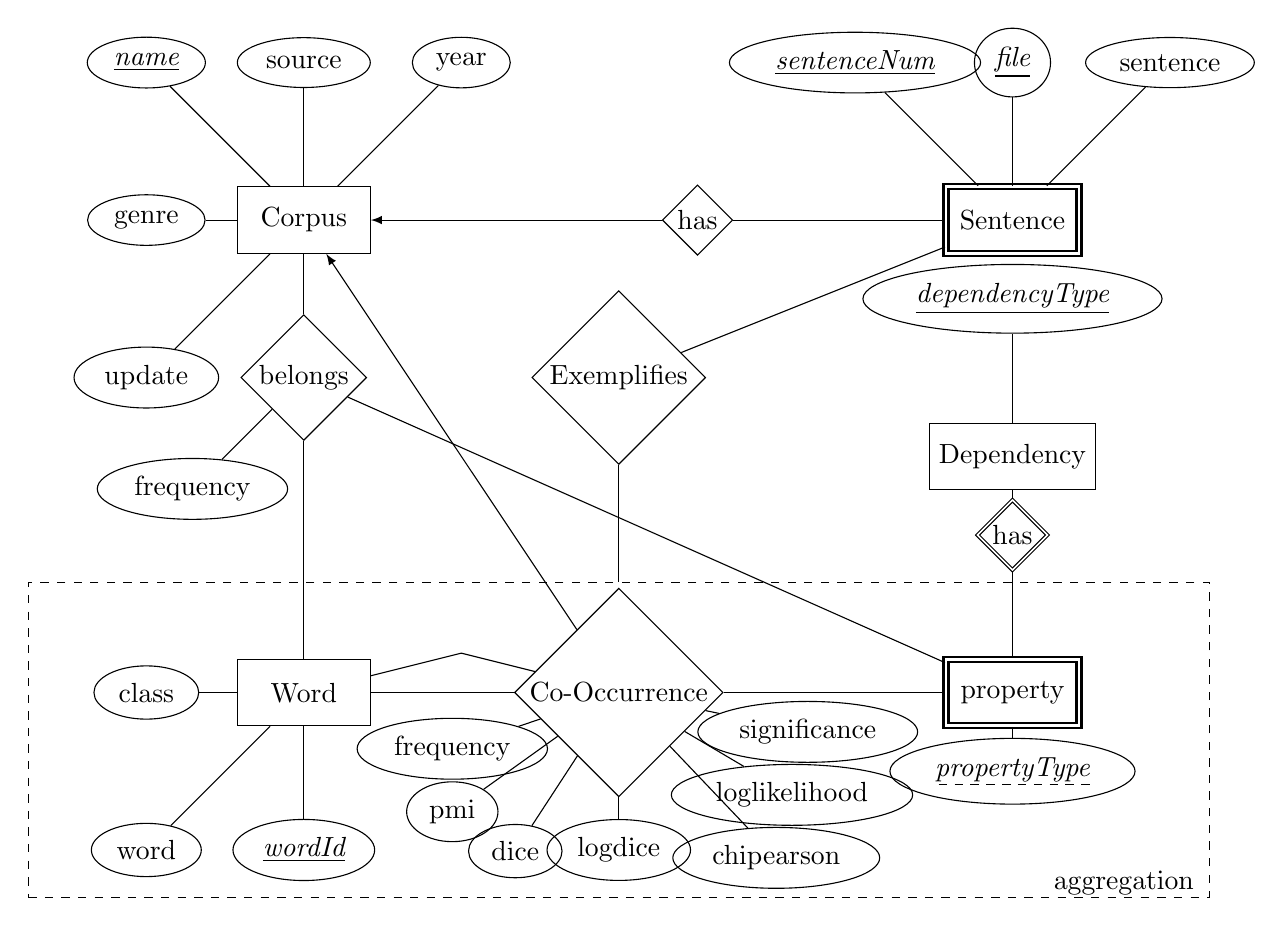
\begin{tikzpicture}[node distance = 2cm, on grid]

  \node [entity] (corpus) {Corpus}
    child {node [attribute, above of=corpus] (csource) {source}}
    child {node [key attribute, left of=csource] (cname) {\underline{name}}}
    child {node [attribute, below of=cname] (cgenre) {genre}}
    child {node [attribute, right of=csource] (cyear) {year}}
    child {node [attribute, below of=cgenre] (cupdate) {update}};

  \node [entity, line width=0.8pt, double, double distance=1pt, right of=corpus, node distance=9cm] (sentence) {Sentence}
    child {node [key attribute, above of=sentence] (sfile) {\underline{file}}}
    child {node [key attribute, left of=sfile] (snum) {\underline{sentenceNum}}}
    child {node [attribute, right of=sfile] (ssentence) {sentence}};

  \node [entity, below of=corpus, node distance=6cm] (word) {Word}
    child {node [key attribute, below of=word] (wid) {\underline{wordId}}}
    child {node [attribute, left of=word] (wclass) {class}}
    child {node [attribute, below of=wclass] (wword) {word}};

  \node [entity, below of=sentence, node distance=3cm] (dependency) {Dependency}
    child {node [key attribute, above of=dependency] {\underline{dependencyType}}};

  \node [entity, line width=0.8pt, double, double distance=1pt, below of=dependency, node distance=3cm] (property) {property}
    child {node [key attribute, below of=property, node distance=1cm] (ptype) {\dashuline{propertyType}}};

  \node [relationship, right of=corpus, node distance=5cm] {has}
    edge [-latex] (corpus)
    edge (sentence);

  \node [relationship, below of=corpus, node distance=2cm] (belongs) {belongs}
    child {node [attribute, below left of=belongs] (bfreq) {frequency}}
    edge (corpus)
    edge (word);

  \node [relationship, double, below of=dependency, node distance=1cm] {has}
    edge (dependency)
    edge (property);

  \node [relationship, right of=word, node distance=4cm] (cooc) {Co-Occurrence}
    edge (property)
    child {node [attribute, below left of=cooc, xshift=-0.7cm, yshift=0.7cm] (freq) {frequency}}
    child {node [attribute, below of=freq, node distance=0.8cm] (pmi) {pmi}}
    child {node [attribute, right of=pmi, node distance=0.8cm, yshift=-0.5cm] {dice}}
    child {node [attribute, below of=cooc] {logdice}}
    child {node [attribute, below of=cooc, xshift=2cm, yshift=-0.1cm] {chipearson}}
    child {node [attribute, below of=cooc, xshift=2.2cm, yshift=0.7cm] {loglikelihood}}
    child {node [attribute, right of=cooc, xshift=0.4cm, yshift=-0.5cm] {significance}};

  \path [draw] (property) -- (belongs);

  \node [draw,dashed, minimum width=15cm, minimum height=4cm] (agg) at ([yshift=-0.6cm]cooc) {};
  \node [below right of=ptype] {aggregation};

  \draw [-latex] (cooc) -- (corpus);
  \draw (cooc) -- (word);
  \draw (cooc) -- (2cm,-5.5cm) -- (word);

  \node [relationship, above of=cooc, node distance=4cm] {Exemplifies}
    edge (sentence)
    edge (agg);

\end{tikzpicture}

\end{figure}

The entities \textit{Corpus}, \textit{Word} and \textit{Dependency} are used to
store the information about each corpus, word and dependency type respectively.

The weak entity \textit{Property} associates the \textit{Dependency} with a
property type.

Each word has a \textit{Belongs} relation with the corpus, which indicates how
often the word occurs in the Corpus.

Each pair of words and property also have a \textit{Co-occurrence} relation,
with a \textit{frequency} attribute which defines how often these words occur
together in the same corpus with the given property. Additionally, several
attributes exist for each kind of association measure.

The weak entity \textit{Sentence} has a \textit{Belongs} association with the
\textit{Corpus}, and the aggregation of the \textit{Co-occurrence} associations
has a \textit{Exemplifies} association with the \textit{Sentence} entity.

Additionally, the following \acp{IC} were identified:

\begin{enumerate}
  \item The words in the \textit{Co-occurrence} association must belong to the
\textit{Corpus} to which they are associated with.
  \item The \textit{Co-occurrence} association must be associated to the same
\textit{Property} with which the words associate with in \textit{Belongs}.
  \item The sentences in the \textit{Exemplifies} association must belong to the
\textit{Corpus} to which the given \textit{Co-occurrence} is associated with.
\end{enumerate}

\subsubsection*{Co-occurrence extraction}

The co-occurrence extractor obtains the processed XML from XIP, and then parses
it to obtain the dependency information.

The extractor reads all dependencies parsed from the XML and stores in the
database, for each:

\begin{itemize}
  \item The type of the dependency in question;
  \item The lemma and class of each word in the dependency;
  \item The property of the dependency;
  \item The sentence in which the dependency occurred.
\end{itemize}

\subsubsection*{Association Measures}
\label{sec:assoc}

After the database is populated with the co-occurrences from the \textit{corpus}
the association measures are calculated in batches of 2,000 co-occurrences
each.

The measures calculated are:

\begin{itemize}
  \item \ac{PMI};
  \item \textit{Dice} Coefficient;
  \item \textit{LogDice};
  \item Pearson's Chi-Square Test;
  \item Log Likelihood Ratio;
  \item Significance Measure.
\end{itemize}

\subsection{Information Display}

The extracted information which was stored in the database is then displayed to
the user through the use of a web interface written in \ac{PHP} and AngularJS.
The \emph{front-end}, executed on the \emph{client-side}, makes \ac{AJAX}
requests to the \emph{back-end}, executed on the \emph{server-side}.

% kate: default-dictionary en_GB; indent-width 2; replace-tabs on;
% kate: remove-trailing-space on; space-indent on;
% kate: replace-trailing-space-save on; remove-trailing-space on;

\section{Summary}

Below is a comparison of the various algorithms mentioned in the previous
sections. The algorithms are evaluated according to their performance and to
their features.

\subsection{WSI Algorithms.}

\ac{DSM}-based algorithms have to deal with scalability problems as the number
of contexts increases. Many of them try to deal with the problem by using denser
representations of the context vectors used.

In comparison, graph-based algorithms try to deal with the significance of a
number of co-occurrences, trying to suppress irrelevant co-occurrences as edges
or using smoothing techniques to generate edges, which were not represented in
the original graph.

As it can be seen in Table~\ref{tab:uswsi} and Table~\ref{tab:wsi}, current
implementations of \ac{DSM} and graph-based algorithms have equivalent
performance when compared using either F-score, V-measure or supervised recall.
It is important to note that unless the \ac{GS} and test data used is the same,
the results obtained are not comparable among implementations.

\begin{table}
\caption[Unsupervised evaluation of \acl*{WSI} algorithms]
{Unsupervised evaluation of \ac{WSI} algorithms in nouns. All measures are in
percentage ($\%$). 1c1word, \ac{MFS}, and Random are baselines from each of the
respective datasets. 1c1word and \ac{MFS} groups all instances of a word into a
single cluster.}
\label{tab:uswsi}

\begin{tabu} to \textwidth { Xlrrrrrr }
\hline
\textbf{Algorithm} & \textbf{GS} & \textbf{Prec.} & \textbf{Recall} & \textbf{Purity} & \textbf{Entropy} & \textbf{F-score} & \textbf{V-measure} \\
\hline
CBC               & WordNet        & 60.8 & 50.8 & ---  & ---  & 55.4 & ---  \\
Widdows and Dorow & WordNet        & ---  & ---  & 82.0 & ---  & ---  & ---  \\
Collocations-JC   & \ac{SWSI} 2007 & ---  & ---  & 88.6 & 31.0 & 78.0 & ---  \\
Collocations-BL   & \ac{SWSI} 2007 & ---  & ---  & 89.6 & 29.0 & 73.1 & ---  \\
UoY     & WSI\&D 2010    & ---  & ---  & ---  & ---  & 38.2 & 20.6 \\
HERMIT  & WSI\&D 2010    & ---  & ---  & ---  & ---  & 30.1 & 16.7 \\
\hline
1c1word & \ac{SWSI} 2007 & ---  & ---  & ---  & ---  & 80.7 & 
0.0\footnotemark[1] \\
Random  & \ac{SWSI} 2007 & ---  & ---  & ---  & ---  & 38.1 & 
4.9\footnotemark[1] \\
MFS     & WSI\&D 2010    & ---  & ---  & ---  & ---  & 57.0 & 0.0  \\
Random  & WSI\&D 2010    & ---  & ---  & ---  & ---  & 30.4 & 4.2  \\
\hline
\end{tabu}
\end{table}

\footnotetext[1]{The mentioned data points were obtained from
\citep{manandhar2009semeval}.}

\begin{table}
\caption[Supervised evaluation of \acl*{WSI} algorithms]
{Supervised evaluation of \ac{WSI} algorithms. Unless otherwise specified, in
the WSI\&D 2010 dataset, the 80-20 split is used.}
\label{tab:wsi}

\begin{tabu} to \textwidth { XXr }
\hline
\textbf{Algorithm} & \textbf{Testing Corpus} & \textbf{Sup. Recall} (\%)\\
\hline
Collocations-JC           & \ac{SWSI} 2007 & 86.4 \\
Collocations-BL           & \ac{SWSI} 2007 & 85.6 \\
UoY            & WSI\&D 2010    & 59.4 \\
HERMIT           & WSI\&D 2010    & 53.6 \\
\hline
MFS           & WSI\&D 2010    & 53.2 \\
Random        & WSI\&D 2010    & 51.5 \\
\hline
\end{tabu}
\end{table}

\subsection{Graph Clustering Algorithms.}

The work in this area introduces algorithms that are time-linear to the number 
of edges with results comparable to older existing algorithms.

Both algorithms are shown to be suitable for \ac{WSI} tasks. Both algorithms are
time-linear to the number of edges and ideal for execution in large-scale graphs
which feature small-world features, as it can be seen on Table~\ref{tab:clalg}.

\ac{CW} is already frequently used in the area of \ac{WSI} with good results,
but unlike MaxMax, it is not deterministic, and it does not allow to place the
same node in several clusters -- soft-clustering --, a feature specially
desirable for a global graph approach so that one word can have several senses.
On the other hand, MaxMax is known to generate many fine-grained clusters, which
then have to be merged to obtain clusters more similar in size to the target
senses \citep{hope2013uos}.

\begin{table}
\caption[Comparison of Graph Clustering Algorithms]
{Comparison of Graph Clustering Algorithms. Retrieval Precision (rPrec.),
Retrieval Recall (rRecall), F-score and V-measure are measured in percentage
($\%$).}
\label{tab:clalg}

\begin{tabu} to \textwidth {Xllrrrr}
\hline
\textbf{Alg.} & \textbf{Determ.} & \textbf{Soft-Clust.} & \textbf{rPrec.} & \textbf{rRecall} & \textbf{F-sc.} & \textbf{V-mes.} \\
\hline
\acl*{CW} & No            & No              & 94.8 & 71.3 & ---  & ---  \\
MaxMax      & Yes           & Yes             & ---  & ---  & 13.2 & 32.8 \\
\hline
\end{tabu}
\end{table}

% kate: default-dictionary en_GB; indent-width 2; replace-tabs on;
% kate: remove-trailing-space on; space-indent on;
% kate: replace-trailing-space-save on; remove-trailing-space on;


% kate: default-dictionary en_GB; indent-width 2; replace-tabs on;
% kate: remove-trailing-space on; space-indent on;
% kate: replace-trailing-space-save on; remove-trailing-space on;

\chapter{Architecture}
\label{ch:architecture}

In this chapter, the architecture of the \ac{WSI} and \ac{WSD} system is 
presented, as well as its 
articulation with the \ac{STRING} \ac{NLP} system.

The architecture of this system consists of four components, ordered as per
Figure~\ref{fig:architecture}:

\begin{enumerate}
  \item a corpus pre-parser, which prepares the corpus being used to be
processed by \ac{STRING};
  \item the co-occurrence extractor from \citet{correia2015syntax};
  \item a graph constructor and clustering algorithm;
  \item a word sense disambiguation module.
\end{enumerate}

\begin{figure}[ht]
  \caption{The architecture of the system}
  \label{fig:architecture}
  \centering
  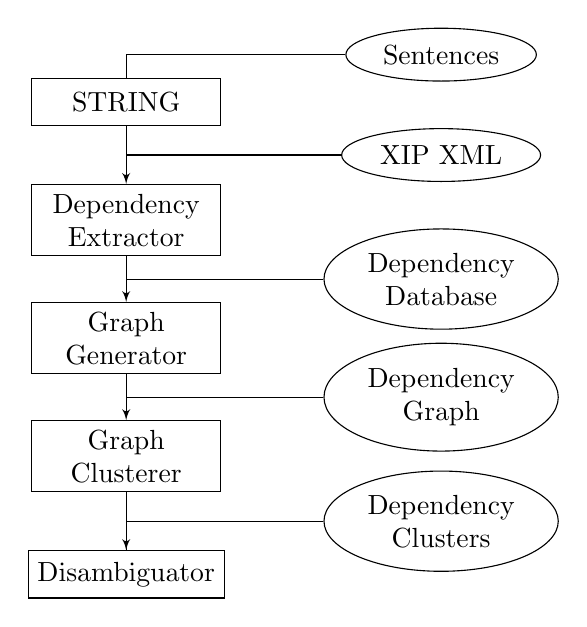
\begin{tikzpicture}[
    on grid,
    node distance = 1.5cm
  ]
  \tikzstyle{block} = [
    draw, rectangle,
    text centered,
    align          = center,
    minimum width  = 2.4cm,
    minimum height = 0.6cm
  ]
  \tikzstyle{data}  = [
    draw, ellipse,
    text centered,
    align          = center,
    node distance  = 4cm
  ]
  \tikzstyle{arrow}  = [draw, -latex']
  \tikzstyle{line}   = [draw]

  \node [block]                         (string)       {STRING};
  \node [block, below of = string]      (depextract)   {Dependency \\ Extractor};
  \node [block, below of = depextract]  (graphgen)     {Graph \\ Generator};
  \node [block, below of = graphgen]    (graphcluster) {Graph \\ Clusterer};
  \node [block, below of = graphcluster] (disambiguator) {Disambiguator};
  
  \path [arrow] (string)     -- coordinate[midway](sd) (depextract);
  \path [arrow] (depextract) -- coordinate[midway](dg) (graphgen);
  \path [arrow] (graphgen)   -- coordinate[midway](gg) (graphcluster);
  \path [arrow] (graphcluster) -- coordinate[midway](gc) (disambiguator);
  
  \node [data] at (4cm,  0.6cm)         (sentences)     {Sentences};
  \node [data, right of = sd]           (xipxml)       {XIP XML};
  \node [data, right of = dg]           (depdb)        {Dependency \\ Database};
  \node [data, right of = gg]           (depgraph)     {Dependency \\ Graph};
  \node [data, right of = gc]           (depcls)       {Dependency \\ Clusters};
  
  \path [line] (sentences) -| (string);
  \path [line] (xipxml) -- (sd);
  \path [line] (depdb) -- (dg);
  \path [line] (depgraph) -- (gg);
  \path [line] (graphcluster) |- (depcls);
  \path [line] (graphcluster) -- (disambiguator);
\end{tikzpicture}

\end{figure}

The data flow is represented in Figure~\ref{fig:data-progression}. The 
processed text from \ac{STRING} 
goes through a modified implementation of the co-occurrence extractor from 
\citet{correia2015syntax}, which stores the co-occurrence word-pairs along with 
their frequencies and association measures' corpora's values in a database.

\begin{figure}[ht]
 \caption{The progression of data as it evolves through the architecture}
 \label{fig:data-progression}
 \centering
 \tikzstyle{block} = [rectangle, draw,
    text width=6em, text centered, minimum height=3em]
\tikzstyle{line} = [draw, -latex']

\begin{tikzpicture}[node distance = 2cm, on grid]
    % Place nodes
    \node [block] (init) {POS-tagged paragraphs};
    \node [block, below of=init] (pairs) {word pairs};
    \node [block, below left of=pairs, node distance=3cm] (nodes) {nodes};
    \node [block, below right of=pairs, node distance=3cm] (edges) {edges};
    \node [block, below right of=nodes, node distance=3cm] (cooc) {co-occurrence graph};
    \node [block, below of=cooc, node distance=2.5cm] (cluster) {cluster of nodes};

    \path [line] (init) -- (pairs) node [midway, right] {co-occurrence extraction};
    \path [line] (pairs) -| (nodes) node [near end, left] {words};
    \path [line] (pairs) -| (edges) node [near end, right] {relations};
    \path [line] (nodes) |- (cooc);
    \path [line] (edges) |- (cooc);
    \path [line] (cooc) -- (cluster) node [near end, right] {clustering algorithm};

    \draw ($(nodes.north west) + (-0.5,0.5)$) rectangle ($(cooc.south east) + (2.6,-0.5)$);
    \node [below left of=cooc, xshift=-1cm] () {graph construction};
\end{tikzpicture}

\end{figure}

\section{Co-occurrence Extraction and Storage}

Syntactic co-occurrences are extracted using the work by
\citet{correia2015syntax}, as per the example in Figure~\ref{fig:orange-example}. Additionally, this work uses the named entities
obtained from \ac{XIP}. If the word in a co-occurrence is a named entity, the
lemma of the word is attributed with the appropriate category (for example, the
word \emph{Pedro} is identified with the lemma \texttt{INDIVIDUAL}).

\begin{figure}[ht]
  \caption{Example of the co-occurrences extracted from a sample sentence}
  \label{fig:orange-example}
  \centering
  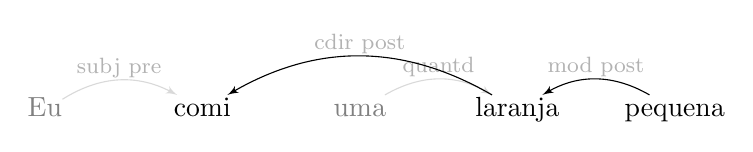
\begin{tikzpicture}[
    on grid,
    node distance = 2cm,
    font = \normalsize
  ]

  %\clip (-0.175cm,-0.175cm) rectangle (7.0cm,0.9cm);

  \tikzstyle {every node} = [color = gray, text height = 1.8ex, text depth = 0.55ex, inner sep = 0]
  \tikzstyle {every path} = [color = gray!30!white, draw=gray!30!white, -latex']
  \tikzstyle {lbl} = [font = \footnotesize, color = gray!60!white, inner sep=0]

  \node (0) {Eu};
  \node [color=black, base right = of 0] (1) {comi};
  \node [right of = 1] (2) {uma};
  \node [color=black, base right = of 2] (3) {laranja};
  \node [color=black, base right = of 3] (4) {pequena};


  \draw (0) to [bend left] node[lbl, above] {subj pre} (1);
  \path (2) to[bend left] node[lbl, above] {quantd} (3);
  \path [draw, color=black] (3) to[bend right] node[lbl, above] {cdir post} (1);
  \path [draw, color=black] (4) to[bend right] node[lbl, above] {mod post} (3);
\end{tikzpicture}

% kate: default-dictionary pt_PT; indent-width 2; replace-tabs on;
% kate: remove-trailing-space on; space-indent on;
% kate: replace-trailing-space-save on; remove-trailing-space on;

\end{figure}


The co-occurrences are then stored in an SQLite database, using the \ac{ER} model in
Figure~\ref{fig:er-model}, adapted from \citet{correia2015syntax}, with minor 
changes to keep information of all the sentences used (in the \emph{Context}
entity) instead of only 20 randomly selected sentences for each co-occurrence.

\begin{figure}[ht]
    \caption{The \acl*{ER} model used to store the information in the database}
    \label{fig:er-model}
    \centering
    \tikzstyle{every node}=[font=\small]
%\tikzstyle{every entity}=[]
\tikzstyle{every attribute}=[font=\small]

\tikzstyle{weak entity}=[entity, line width=0.8pt, double, double distance=1pt]
\tikzstyle{weak relationship}=[relationship, double, double distance=1pt]

\begin{tikzpicture}[node distance = 2cm, on grid]
  \node [entity] (corpus) at (0,0) {Corpus}
    child {node [key attribute] (cname) at (1,1.5) {\underline{name}}}
    child {node [attribute] (csource) at (-1,3) {source}}
    child {node [attribute] (cyear) at (-1,3) {year}}
    child {node [attribute] (cgenre) at (-1,3) {genre}}
    child {node [attribute] (cupdate) at (-1,3) {update}};

  \node [weak entity] (file) at (4,0) {File}
    child {node [key attribute] (fname) at (0,3) {\dashuline{name}}};

  \node [entity] (word) at (0,-5) {Word}
    child {node [key attribute] (wword) at (-1,2) {\underline{word}}}
    child {node [key attribute] (wclass) at (-2.5,1) {\underline{class}}};

  \node [weak entity] (context) at (8,0) {Context}
    child {node [key attribute] (csentence) at (0,3) {\dashuline{sentence}}};

  \node [entity] (dependency) at (8,-1.5) {Dependency}
    child {node [key attribute] (dtype) at (2,1.5) {\underline{type}}};

  \node [weak entity] (property) at (8,-5) {Property}
    child {node [key attribute] (ptype) at (2,1.5) {\dashuline{type}}};

  \node [relationship] (co-occurrence) at (4,-5) {co-occurrence}
    edge [-latex] (word)
    edge [-latex] (property)
    edge [-latex] (corpus)
    child {node [attribute] {frequency}}
    child {node [attribute] {pmi}}
    child {node [attribute] {npmi}}
    child {node [attribute] {dice}}
    child {node [attribute] {logDice}}
    child {node [attribute] at (0,-0.5) {chiPearson}}
    child {node [attribute] {logLikelihood}}
    child {node [attribute] at (0,-0.5){significance}};

  \draw [-latex] (co-occurrence) -- (2,-4.5) -- (word);

  \node [weak relationship] at (8,-2.8) {has}
    edge [-latex] (dependency)
    edge [line width=0.8pt, double, double distance=1pt] (property);

  \node [relationship] at (0,-2) {belongs}
    edge [-latex] (corpus)
    edge [-latex] (property)
    edge [-latex] (word)
    child {node [attribute] (bfreq) at (-2.5,1.5) {frequency}};

  \node [weak relationship] at (2,0) {has}
    edge [-latex] (corpus)
    edge [line width=0.8pt, double, double distance=1pt] (file);

  \node [weak relationship] at (6,0) {has}
    edge [-latex] (file)
    edge [line width=0.8pt, double, double distance=1pt] (context);

  \node [draw,dashed, minimum width=15cm, minimum height=3.6cm] (agg) at ([yshift=-0.5cm]co-occurrence) {};

  \node [relationship] at (4,-2) {occurs}
    edge [-latex] (agg)
    edge [-latex] (context)
    child {node [attribute] at (2, 1) {frequency}};
\end{tikzpicture}

\end{figure}

Additionally, the relationship \emph{Exemplifies} is replaced with
\emph{Occurs}, which associates all \emph{Co-occurrence} aggregations with all
the respective \emph{Context}s where they occur.

\section{Graph Generation and Clustering}

For a target word $w$, a query to the database is made to obtain the word pairs 
and association measure values of all co-occurrences which occur in the same 
contexts as $w$. After filtering all co-occurrences which do not reach the 
minimum threshold value of the association measure being used, the 
co-occurrences are saved in a graph structure.

To ensure that only words directly related to $w$ remain, a breadth-first 
search is made starting from the target word. Only the nodes which were visited 
during this process are kept in the final graph.

After the graph is generated, a graph clustering algorithm is run against it,
and the resulting senses are stored.

\section{Sense Disambiguation}

Disambiguation is done by measuring the separation between the words in the
given context and each of the induced sense clusters. The sense with the lowest
separation score is the most likely sense of the word.

For a target word $w$ from a given context $c$, the co-occurrences from $c$ are
extracted and used to generate the cluster for the context, $C_i$.

Then, for each inferred sense cluster $C_j$ of $w$, the
\emph{Separation} between $C_i$ and $C_j$ is calculated according to
Equation~\ref{eq:separation} \citep{hope2013uos}. $\operatorname{proximity}$ is
defined as the weight of the co-occurrence in the dependency graph of the word.

\begin{equation}
 \operatorname{separation}(C_i,C_j) =
 1 - \left(
 \frac {\sum_{\substack{x \in C_i \\ y \in C_j}} \operatorname{proximity}(x,y)}
       {|C_i| \times |C_j|}
 \right)
\label{eq:separation}
\end{equation}

The cluster $C_j$ with the lowest separation score compared to $C_i$ is then
considered the most likely sense of the target word $w$.


% kate: default-dictionary en_GB; indent-width 2; replace-tabs on;
% kate: remove-trailing-space on; space-indent on;
% kate: replace-trailing-space-save on; remove-trailing-space on;

\chapter{Implementation}
\label{ch:implementation}

\section{Corpora Pre-Parse}

Two \emph{corpora} were chosen to be used in this project, the CETEMPúblico 
\emph{corpus} \citep{rocha2000cetempublico}, and a dump of the Portuguese 
edition of Wikipedia 
\footnote{\url{https://en.wikipedia.org/wiki/Wikipedia:Database_download}, last
accessed on \DTMdate{2017-06-21}.}. Each \emph{corpus} used its own syntax to
describe its contents. As \ac{STRING} only parses plain text sentences, the
additional meta-data provided was either removed or adapted for parsing by
\ac{STRING}.

\subsection{CETEMPúblico}

CETEMPúblico was provided in \ac{SGML} format with the following tags:

\begin{description}[labelwidth=3em]
 \item [\texttt{ext}] Extract (usually composed of two paragraphs);
 \item [\texttt{p}]   Paragraph;
 \item [\texttt{s}]   Sentence;
 \item [\texttt{t}]   Title;
 \item [\texttt{a}]   Author;
 \item [\texttt{li}]  List element.
\end{description}

To parse it, a Python script was designed, which parses it as \ac{XML} using a
parser that generates the element tree incrementally. Tags considered
irrelevant were ignored, and tags with special meanings, such as the ones
setting the boundaries of a sentence, paragraph or excerpt were replaced with
unique plain text identifiers.

Because the corpus was in \ac{SGML} format and not \ac{XML}, a few replacements
were made before feeding each line to the parser to make sure that the parser 
would only be fed valid \ac{XML}. These made sure attributes were quoted and 
that all elements had an opening and closing tag.

\subsection{Wikipedia}

After obtaining the Wikipedia dump, a tool called WikiExtract
\footnote{\url{https://github.com/attardi/wikiextractor}, last accessed on
\DTMdate{2017-06-21}.} was used to convert the obtained \ac{XML} into mostly
plain text files.

Further cleaning was executed, in which all possible invalid \ac{XML} or
possible leftover tags were found using a regular expression, added to a list,
and removed automatically.

At last, document boundaries and paragraphs were replaced with unique
plain text identifiers which can be recognized even after being parsed by
\ac{STRING}.

\section{Co-occurrence Extraction}

To obtain the co-occurrences, the extractor created by \citet{correia2015syntax}
was used, but had to be adapted because it had been developed under different
requirements and conditions distinct from the ones for this work.

\subsection{Storage Model}

To be able to provide all the required information to the graph construction
algorithm, the model used to store the information had to be modified. A new 
\ac{ER} was designed, as shown in Figure~\ref{fig:er-model}, and used to
generate the relational model used in the database.

All tables have their own \texttt{id}, used as the primary key, with the 
previous primary key being set with a \texttt{UNIQUE} constraint. The new 
\texttt{id} primary key is used to reference to a given table's line in other 
tables. This helped to reduce the space occupied by repeated references to 
text-based primary keys.

\subsection{Parsing \ac{XIP} files}

The \ac{XIP} files were being parsed as XML using Java's W3C based \ac{DOM}
parser\footnote{\url{https://docs.oracle.com/javase/8/docs/api/org/w3c/dom/package-summary.html},
last accessed on \DTMdate{2017-08-06}}. This parser loads the file in memory and
creates the \ac{DOM}-like tree structure from there.

This implementation was having problems with larger files, on the range of
100MB and larger, taking exponential amounts of time to perform the most basic
operations.

The existing \ac{DOM} parser was thus replaced with a pull-parser. This reads
the file sequentially and, as new tags are found, such as the start or the
end of an element, an event is generated, with only the contents pertaining to 
it.

The pull-parser has an $O(1)$ memory usage for parsing, as only the currently
parsed segment needs to stay in memory while the document structure is built.

On top of the XML pull parser, a basic stack is used to keep track of what is
the current element and depth in the document. The name of the current tag
is pushed to the stack when a start event is emitted, and the top element is
popped when an end event is emitted.

With the events and the stack, a state machine is used, which is responsible for
deciding the next action in the construction of the XIP document in memory.

\subsection{Populating the Database}

After parsing the \ac{XIP} files, the dependencies are extracted and added to 
the database as co-occurrences. First an \texttt{INSERT} is attempted, if it 
fails due to \texttt{UNIQUE} violations, the existing entry is updated with the 
new information.

After all co-occurrences are added to the database, the values of the
association measures are updated in batches of 2000 at a time. To prevent
slowdowns while waiting to read, a cache of read values from the database is
used to prevent reading multiple times the same value from the database,
allowing to reduce considerably the time taken to populate the values of the 
association measures.

\section{Sense Induction}

Given a target word $w$, a query to the database is made to obtain all
co-occurrences that happen in the same context as co-occurrences with $w$ as
either the first or second word, as in Listing~\ref{lst:contextextract}.

\begin{lstlisting}[language=SQL,float=h,caption=SQL Query to extract all
co-occurrences in same context as the target word,label=lst:contextextract]
SELECT Coocorrencia.*,
       p1.palavra AS p1lemma,
       p1.classe AS p1class,
       p2.palavra AS p2lemma,
       p2.classe AS p2class
FROM Coocorrencia
INNER JOIN CoOccurrenceContexts ON Coocorrencia.id = CoOccurrenceContexts.cooccurrence
INNER JOIN Palavra AS p1 ON Coocorrencia.idPalavra1 = p1.idPalavra
INNER JOIN Palavra AS p2 ON Coocorrencia.idPalavra2 = p2.idPalavra
WHERE CoOccurrenceContexts.context IN
    ( SELECT CoOccurrenceContexts.context
     FROM CoOccurrenceContexts
     INNER JOIN Coocorrencia ON CoOccurrenceContexts.cooccurrence = Coocorrencia.id
     WHERE Coocorrencia.idPalavra1 = ?1
       OR Coocorrencia.idPalavra2 = ?1)
\end{lstlisting}

The resulting set of rows consists of all co-occurrences happening in the same
context as $w$. These are then assembled into a graph, in which all the nodes
represent the words from the set, and the edges represent the co-occurrences of
that same set.

All co-occurrences in which the association measure's weight is lower than a
pre-specified threshold are then removed from the graph.

A breadth-first search is then applied, starting from $w$, to ensure that only 
nodes directly connected to $w$ by any number of steps remain in the graph. This
eliminates nodes and co-occurrences not connected to the graph at all, coming
-- for example -- from dangling co-occurrences that were previously connected
through a path removed in one of the previous steps of the generation.

The resulting graph is finally clustered using the \ac{CW} algorithm, explained
in Section~\ref{sec:clusteralgorithms}.

\section{Sense Disambiguation}

To be able to perform disambiguation, additional changes had to be done to the
co-occurrence extractor in \citep{correia2015syntax}. The extractor had the 
logic
to extract the co-occurrences and the code to write them in the database merged
together. To make the extractor usable for the task of disambiguation, a
separation of the code to write in the database and the logic of extracting the
co-occurrences was performed.

Having applied those changes, the disambiguation for a target word $w$ and a
context $c$ starts by using the modified extractor to obtain all co-occurrences
which occur in $c$. These are considered the cluster of co-occurrences of the
word $w$ in context $c$.

To discover which of the induced senses $s$ is the most likely to be in use,
each one of them is compared to the cluster of co-occurrences from the context
using the measure of \emph{separation} defined in Equation~\ref{eq:separation}.
The cluster with the lowest \emph{separation} is considered the most likely
sense of the word in the given context.

\section{Avoiding Duplicated Calculations}

As many of these steps can take considerable amounts of time, it is desirable to
avoid repeating them as often as it is possible. As a result, most of the
execution pipeline of the code was adapted to read and write from files as often
as possible, allowing the project to use these files as a cache for calculated
operations.

The format chosen was a subset of \ac{CSV} files, in which each element was a
row and each property was a column.

Each time an extensive operation is concluded, such as obtaining the
co-occurrences in the context of a word, or generating the clusters for a
word using a given set of parameters, the results are saved in a CSV file.

If that same set of data is required later on, instead of re-calculating it
from scratch, the information is obtained from the existing file.

% kate: default-dictionary en_GB; indent-width 2; replace-tabs on;
% kate: remove-trailing-space on; space-indent on;
% kate: replace-trailing-space-save on; remove-trailing-space on;

\chapter{Evaluation}
\label{ch:eval}

\chapter{Evaluation Methodology}

The evaluation is composed of two methods, an unsupervised evaluation and a
supervised evaluation. The unsupervised evaluation is used to assess the
resulting clusters' similarity to the \ac{GS} senses. The supervised evaluation
is used as an application-oriented assessment of the resulting clusters in the
task of \ac{WSD}.

\section{Test Corpus}

To evaluate the project, the corpus from \cite{pires2017verb} was used. This was
the PAROLE corpus \cite{nascimento1998parole}, with each verb manually annotated
with its ViPEr class and reviewed by linguists.

\section{Unsupervised Evaluation}
\label{sec:unsupeval}

In this evaluation method, the set of resulting clusters is compared to a
\ac{GS}. This comparison is made by evaluating the clusters'
\textit{homogeneity} and \textit{completeness}. Homogeneity refers to the degree
that each cluster consists of data points primarily belonging to a single
\ac{GS} class. Completeness refers to the degree that each \ac{GS} class
consists of data points assigned to a single cluster
\cite{manandhar2009semeval}. To evaluate homogeneity and completeness, the
F-score and the V-measure will be used.

Given a particular \ac{GS} sense $gs_i$ of size $a_i$ and a cluster $c_j$ of
size $a_j$, the F-score of $gs_i$ and $c_j$ is the harmonic mean of its
precision and its recall, as defined in Equation~\ref{eq:smallf}
\cite{agirre2007semeval}. Precision of a class $gs_i$ with respect to cluster
$c_j$ is the number of common instances divided by total cluster size, i.e.
$P(gs_i, c_i) = \frac{a_{ij}}{a_j}$. The recall of a class $gs_i$ with respect
to cluster $c_j$ is the number of common instances divided by total sense size,
i.e. $R(gs_i, c_j) = \frac{a_ {ij}}{a_i}$.

\begin{equation} \label{eq:smallf}
 f(gs_i, c_j) = \frac{2P(gs_i,c_j)R(gs_i,c_j)}
                     {P(gs_i,c_j) + R(gs_i,c_j)}
\end{equation}

The F-score of a class $gs_i$ is the maximum F-score obtained at any cluster, as
according to Equation~\ref{eq:fscoregs}. The F-Score of the entire clustering
solution is the weighted average of the F-scores of each \ac{GS}, as in
Equation~\ref{eq:fscore}, where $q$ is the number of \ac{GS} senses and $N$ is
the total number of target word instances.

\begin{equation} \label{eq:fscoregs}
 F(gs_i) = \underset{c_j}{\max} f(gs_i, c_j)
\end{equation}

\begin{equation} \label{eq:fscore}
 FS = \sum_{i=1}^q \frac{|gs_i|}{N}F(gs_i)
\end{equation}

The F-score measures both homogeneity (precision) and completeness (recall).
However, the F-score suffers from the \textit{matching problem}, by not
evaluating the entire membership of a cluster \cite{rosenberg2007v}. This is
due to the F-score not considering the components of the clusters beyond the
majority class. Furthermore, the F-score penalises systems for getting the
number of \ac{GS} classes wrongly \cite{manandhar2009semeval}.

Thus, to complement the F-score, the V-measure is also used. V-measure is an
entropy-based measure that explicitly measures how successfully the criteria
of homogeneity and completeness have been satisfied \cite{rosenberg2007v}. Just
as precision and recall are combined to form the F-score, homogeneity and
completeness are combined using the harmonic mean to compute the V-measure.

For the homogeneity criterion, a clustering must assign only the data points of a
single class to a single cluster. That is, the class distribution of each
cluster should be skewed to a single class, zero entropy \cite{rosenberg2007v}.
In a perfectly homogeneous case, $H(GS|C) = 0$ and in an imperfect situation,
this value is dependent on the size of the dataset and distribution of class
sizes. Therefore, the V-measure normalizes this value by the maximum reduction
in entropy the clustering could provide, $H(GS)$, resulting in
Equation~\ref{eq:homogeneity}.

\begin{equation} \label{eq:homogeneity}
 h = \begin{dcases}
      1,                        & \text{if } H(GS,C) = 0 \\
      1 - \frac{H(GS|C)}{H(GS)},& \text{otherwise} \\
     \end{dcases}
\end{equation}

\begin{equation}
 H(GS) = - \sum_{i=1}^{|GS|} \frac{\sum_{j=1}^{|C|} a_{ij}}{N}
         \log \frac{\sum_{j=1}^{|C|} a_{ij}}{N}
\end{equation}

\begin{equation}
 H(GS|C) = - \sum_{j=1}^{|C|} \sum_{i=1}^{|GS|} \frac{a_{ij}}{N}
           \log \frac{a_{ij}}{\sum_{k=1}^{|GS|} a_{kj}}
\end{equation}

Symmetrically to homogeneity, for the completeness criterion, a clustering
solution must assign all of the datapoints of a single class to a single
cluster. This can be evaluated by calculating the conditional entropy of the
proposed cluster distribution given the class of the component data points,
$H(C|GS)$. In a perfectly complete case, $H(C|GS) = 0$ and in the worst case
scenario each class is represented by every cluster with a distribution equal to
the distribution of cluster sizes, $H(C|GS)$ is maximal and equals $H(C)$.
Therefore, adding a way symmetric to that used for homogeneity, the V-measure
defines completeness as in Equation~\ref{eq:completeness}.

\begin{equation} \label{eq:completeness}
 c = \begin{dcases}
      1,                        & \text{if } H(C,GS) = 0 \\
      1 - \frac{H(C|GS)}{H(C)}, & \text{otherwise} \\
     \end{dcases}
\end{equation}

\begin{equation}
 H(C) = - \sum_{j=1}^{|C|} \frac{\sum_{i=1}^{|GS|} a_{ij}}{N}
        \log \frac{\sum_{i=1}^{|GS|} a_{ij}}{N}
\end{equation}

\begin{equation}
 H(C|GS) = - \sum_{i=1}^{|GS|} \sum_{j=1}^{|C|} \frac{a_{ij}}{N}
           \log \frac{a_{ij}}{\sum_{k=1}^{|C|} a_{ik}}
\end{equation}

Based on these calculations of homogeneity and completeness, the V-measure of a
clustering solution is then computed using the weighted harmonic mean of
homogeneity and completeness, according to Equation~\ref{eq:vmes}, in which if
$\beta$ is greater than 1 completeness is weighted more strongly and if less
than 1 homogeneity is weighted more strongly.

\begin{equation} \label{eq:vmes}
 V_\beta = \frac{(1+\beta)hc}{(\beta h) + c}
\end{equation}

Although the V-measure does not increase monotonically, it is known to tend to
favour systems producing a higher number of clusters than the number of \ac{GS}
senses \cite{manandhar2010semeval}. With this in mind, both the F-score and the
V-measure are used for this evaluation method, as the F-score penalises systems
when they produce a different number of clusters from the number of \ac{GS}
senses.

Additional measures for unsupervised evaluation include \textit{entropy} and
\textit{purity}. Entropy measures how various classes of objects are
distributed within each cluster. Generally, the smaller the entropy, the better
the clustering algorithm preforms. On the other hand, Purity measures the extent
to which each cluster contains objects from primarily one class. The larger the
purity, the better the clustering algorithm preforms. A formal definition of
these measures is available in \cite{zhao2005hierarchical}. However, as both of
them evaluate only the homogeneity of a clustering algorithm, disregarding
completeness \cite{manandhar2009semeval}, and are not frequently used in the
evaluation of more recent algorithms, they will not be considered in this
evaluation.

\section{Supervised Evaluation}
\label{sec:supeval}

In the supervised evaluation method, the target corpus is split into a testing
and training part. The training part is used to map the automatically induced
clusters to \ac{GS} senses \cite{agirre2006evaluating}. After that, the testing
corpus is used to evaluate the clustering resulting in a \ac{WSD} setting.

Suppose there are $m$ clusters and $n$ senses for the target word. $M$ is the
set of probabilities of words belonging to clusters, $M = \{m_{ij}\}$, $1 \leq i
\leq m, 1 \leq j \leq n$ and each $m_{ij} = P(gs_j|c_i)$, that is, $m_{ij}$ is
the probability of a word sense $j$ given it that has been assigned to a cluster
$i$. This probability can be computed counting the times an occurrence with
sense $j$ has been assigned to cluster $i$ in the train corpus.

The matrix $M$ is then used to transform any cluster score vector $\overline{h}$
returned by the algorithm into a sense vector $\overline{s}$. This is done by
multiplying the score vector by the matrix $M$, that is, $\overline{s} =
\overline{h}M$.

The mapping matrix $M$ is used in order to convert the cluster score vector
$\overline{h}$ of each test corpus instance into a sense score vector
$\overline{s}$, and then assign the sense with maximum score to that instance.

As the algorithm always returns an answer, its recall is of 100\% in all
cases, there are no false negatives as there aren't any negatives at all. So
the algorithm only needs to be evaluated according to its precision
\cite{agirre2006evaluating}.

% kate: default-dictionary en_GB; indent-width 2; replace-tabs on;
% kate: remove-trailing-space on; space-indent on;
% kate: replace-trailing-space-save on; remove-trailing-space on;


\section{Test Corpus}

To evaluate the project, the corpus from \citep{baptista2013viper} was used. 
This was the PAROLE corpus \citep{nascimento1998parole}, with each verb 
instance manually annotated with its ViPEr class and reviewed by linguists. The 
splitting used for evaluation was to use the whole corpus for training,
except for the sentence being evaluated.

\section{Parameter choosing}

The graph partitioning algorithm chosen was \ac{CW}, as the other option,
MaxMax, has a tendency to generate many fine-grained clusters
\citep{hope2013uos}.

The \ac{NPMI} and the logDice association measures were chosen as due to their
normalized scores, which allow to use the same parameter between different words
while keeping the same underlying meaning. The \ac{NPMI} association measure 
was tested with minimum thresholds of 0.0, 0.25, 0.5, and 0.75, ranging from 
each word being at best independent of the other up to both occurring mostly 
together. The logDice association measure was tested with minimum thresholds of 
0.0, 2.5, 5.0, 7.5, and 10.

\section{Unsupervised Evaluation}

The results of the unsupervised evaluation (Table~\ref{tab:unsup-results}) show 
that all tests scored poorly in F-Score, while \ac{MFS} had a result on average 
of 83.4\%. In the V-Measure, results varied from 0.0\% for the lowest values up 
to 34.4\% for the highest. Not counting the most restrictive threshold of 
logDice and NPMI, all tests had better results than \ac{MFS}, which scored 
0.4\% in V-Measure.

Another thing which is possible to see if that not enough points are available
to form a meaningful view of the contexts when the threshold is too high,
resulting in no clusters at all and giving poor results.

When evaluating the number of clusters, it is possible to see that most tests
might have been penalised due to the high number of clusters they had compared
to the average number of \ac{GS} senses.

\begin{table}[ht]
\caption{Results of the unsupervised \ac*{WSI} evaluation.}
\label{tab:unsup-results}
\begin{tabu} to \textwidth {Xlrrrr}
\hline
\textbf{Algorithm} & \textbf{Association Measure} & \textbf{Threshold} & \textbf{F-Score (\%)} & \textbf{V-Measure (\%)} & \textbf{\# Clusters} \\
\hline
\ac{CW} & logDice   &  0.0 &  1.95 & 33.62 & 147.3 \\
\ac{CW} & logDice   &  2.5 &  1.80 & 33.46 & 252.2 \\
\ac{CW} & logDice   &  5.0 &  2.46 & 29.60 & 259.7 \\
\ac{CW} & logDice   &  7.5 &  2.70 & 18.26 &  48.8 \\
\ac{CW} & logDice   & 10.0 &  0.83 &  3.33 &   0.1 \\
\hline
\ac{CW} & \ac{NPMI} & 0.0  &  2.34 & 30.97 &  76.5 \\
\ac{CW} & \ac{NPMI} & 0.25 &  1.69 & 34.37 & 380.1 \\
\ac{CW} & \ac{NPMI} & 0.5  &  0.72 &  9.80 &   0.2 \\
\ac{CW} & \ac{NPMI} & 0.75 &  0.00 &  0.00 &   0.0 \\
\hline
\ac{MFS} &      --- &  --- & 83.36 &  0.37 &   1.0 \\
\hline
\end{tabu}
\end{table}

\section{Supervised Evaluation}

The results on supervised \ac{WSD} (seen in Table~\ref{tab:sup-results}) were
very poor overall. None of the tests were able to surpass the results of
\ac{MFS}, with a precision of 65.7\%. The highest result was using logDice with
a threshold of 7.5, which reached a precision of 10.1\%.

\begin{table}[ht]
\caption{Results of the supervised \ac*{WSD} evaluation.}
\label{tab:sup-results}
\begin{tabu} to \textwidth {Xlrr}
\hline
\textbf{Algorithm} & \textbf{Association Measure} & \textbf{Threshold} & \textbf{Precision (\%)} \\
\hline
\ac{CW} & logDice   &  0.0 &  5.37 \\
\ac{CW} & logDice   &  2.5 &  0.00 \\
\ac{CW} & logDice   &  5.0 &  8.27 \\
\ac{CW} & logDice   &  7.5 & 10.10 \\
\ac{CW} & logDice   & 10.0 &  2.55 \\
\hline
\ac{CW} & \ac{NPMI} & 0.0  &  0.22 \\
\ac{CW} & \ac{NPMI} & 0.25 &  2.65 \\
\ac{CW} & \ac{NPMI} & 0.5  &  0.00 \\
\ac{CW} & \ac{NPMI} & 0.75 &  0.00 \\
\hline
\ac{MFS} & ---      &  --- & 65.74 \\
\hline
\end{tabu}
\end{table}

\section{Result interpretation and evaluation}

Overall, the tests had poor results. In all examples \ac{MFS} was able to
achieve better results, showing the project is not ready to be used for
disambiguation.

The high number of clusters obtained (on average above the hundreds) shows that
the results are too fine-grained to be able to properly match them to the senses
trying to disambiguate.

Further inspection into specific graphs of some words, such as the graph for the
word \emph{vingar} (Figure~\ref{fig:vingar_graph}) can further explain the
obtained results.

\begin{figure}[ht]
  \caption{Image of the induction graph for the word \emph{vingar}, using the
    \ac*{CW} algorithm and the \ac*{NPMI} association measure.}
  \label{fig:vingar_graph}
  \centering
  \includegraphics[width=\textwidth]{graphics/vingar_VERB_npmi_0_4_chineseWhispers}
\end{figure}

The first noticeable thing is that the graph includes many words with spelling
errors. As these are exceptional, when they do appear, association measure
values rank them as words highly related to the target word, and add noise to
the induction phase.

The second noticeable thing is that although the work by
\citet{correia2015syntax} identifies named entities and replaces their lemmas
with their categories, many of the words in the graph are named entities which
were not recognized by \ac{STRING}. This adds noise to the graph, increasing the
number of small clusters generated.

But the most noticeable thing is how sparse the graph is. Algorithms such as
\ac{CW} or MaxMax require a \emph{small-world network} with several high-density
areas to be able to find clusters in the graph. In a graph such as the one
in Figure~\ref{fig:vingar_graph}, with the exception of the node corresponding
to the target word, no nodes have more than 2 neighbours. This undermines the
assumptions used in graph-clustering algorithms, and prevents the possibility
of better results.

It is possible the graph was sparse because the syntactic dependencies used
impose a stricter relationship between the two words than the usage of mere
words which co-occur in the same sentence or paragraph would. The stricter
relationship between the words changes the behaviour of the resulting graph,
which make the graph-clustering algorithms behave poorly.

Additionally, the stricter relationship might be preventing words that are
related but do not have a syntactic relationship from being included in the
graph. This might make the generated graphs unsuitable for the specific \ac{WSI}
algorithms used in this project.

% kate: default-dictionary en_GB; indent-width 2; replace-tabs on;
% kate: remove-trailing-space on; space-indent on;
% kate: replace-trailing-space-save on; remove-trailing-space on;

\chapter{Conclusion}
\label{ch:conclusion}

This project proposed an algorithm for disambiguating the sense of words in the
Portuguese language without the need to manually create a sense inventory or
sense-tagged corpora. Additionally, this project implemented a proof-of-concept
of this same proposal, and evaluated its results against a \ac{MFS} baseline.

One future investigation point would be to evaluate the use of relaxed
co-occurrences based on context windows, sentences or even paragraphs, instead
of the syntactic dependency co-occurrences used in this project. This might
influence the characteristics of the generated graphs and improve the
performance of the graph-clustering algorithms.

Another aspect should be to investigate vector-based algorithms. These might be
capable of making use of the dependency information provided by \ac{XIP}, and
might perform better in relation to algorithms blind to this
information, such as the ones used in this project.

Additionally, it might be relevant to investigate porting the data to a graph
database engine. The traditional relational database used requires the use of
multiple \texttt{JOIN}s to execute the required queries. A database with a
native concept of a graph would allow to remove these \texttt{JOIN}s and improve
execution speed.

Although the project was unable to achieve satisfactory results in the
evaluation, it was possible to pinpoint where possible weaknesses are located.
A base model was defined and documented, and it can be used as a base for future
attempts at solving the challenges found.

% kate: default-dictionary en_GB; indent-width 2; replace-tabs on;
% kate: remove-trailing-space on; space-indent on;
% kate: replace-trailing-space-save on; remove-trailing-space on;


% Bibliography
\bibliographystyle{chicago}
\bibliography{refs}

\end{document}
% kate: default-dictionary en_GB; indent-width 2; replace-tabs on;
% kate: remove-trailing-space on; space-indent on;
% kate: replace-trailing-space-save on; remove-trailing-space on;
